\chapter{Literature Review and Related Work}
\label{chap:relatedworks}

Generative AI has seen rapid advancements, particularly in video synthesis and manipulation. 
However, as AI-generated content becomes more sophisticated, concerns over deepfake misuse, copyright violations, 
and data exploitation have risen. Several existing tools attempt to address these challenges, 
but they focus primarily on static image protection rather than video poisoning.

\section{Competitor Analysis}
\label{section:competitor-analysis}

\begin{figure}[h]
    \centering
    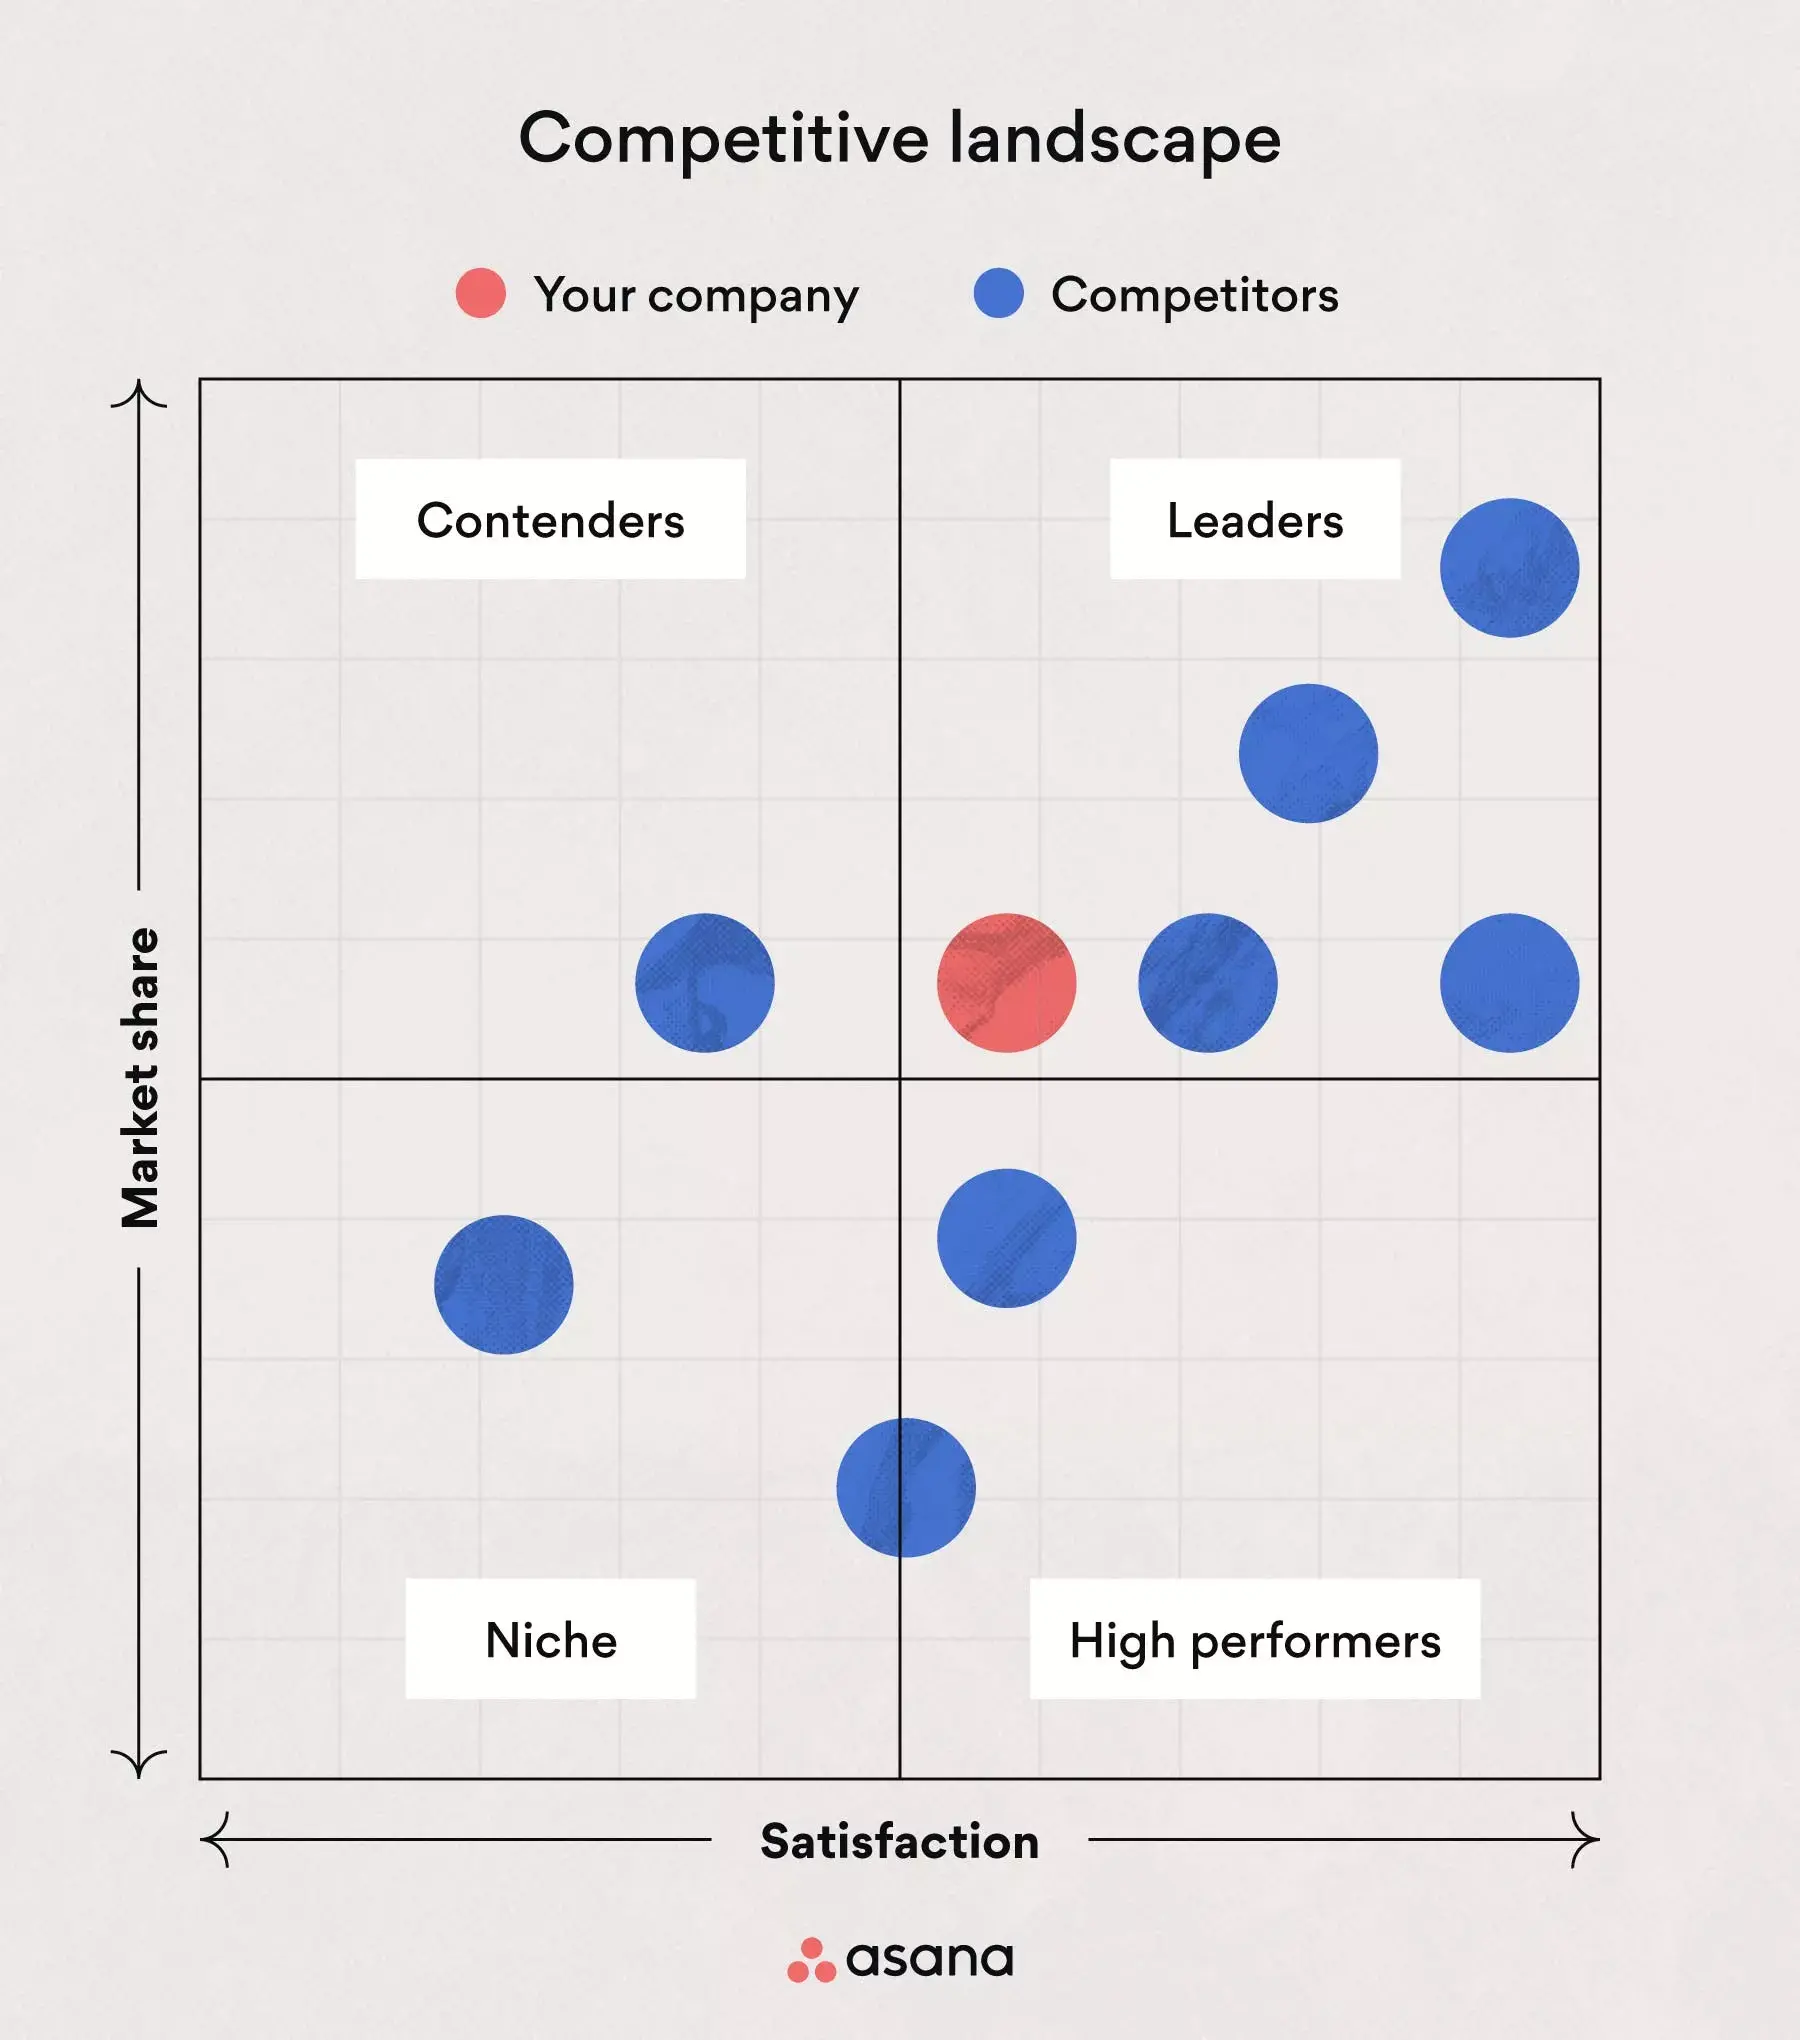
\includegraphics[width=0.5\textwidth]{examples/asana-competitive-landscape.jpg}
    \caption{Competitive Landscape}

    As there are currently no poisoning processor for videos, we'll be comparing to static image poisoning processor as our competitor, in a scenarios where they extract the video's graphics frame by frame, and poison each of them as a static image, and then reassembled them back as a video.

    The goal of the software is to protect the video from AI training by data poisoning method Adversarial attack; to break AI's accuracy by adding information to the data that is imperceptible to the human eye.
    \begin{enumerate}
        \item Glaze
        \item MIST
        \item Anti-Dreambooth
        \item ART : Adversarial Robustness toolbox
    \end{enumerate}

\end{figure}

\section{Literature Review}
\label{section:literature-review}
This project doesn't necessarily create a new poisoning tactics as research, but to optimize our software and be a reliable data security tool, we also have to be familiar with various research.
\begin{enumerate}
    \item stAdv
    \item BTC-UAP
\end{enumerate}